\documentclass{bmvc2k}
\usepackage{graphicx}
\usepackage{amsmath}
\usepackage{amssymb}
\usepackage{mathtools} % mathtools builds on and extends amsmath package
% \usepackage{algorithm}		% http://ctan.org/pkg/algorithms
\usepackage{algpseudocode}	% http://ctan.org/pkg/algorithmicx% Include other packages here, before hyperref.
\usepackage{comment, url}
\usepackage[ruled, vlined, linesnumbered]{algorithm2e}
\newcommand{\forceindent}{\leavevmode{\parindent=1em\indent}}

%% Enter your paper number here for the review copy
\bmvcreviewcopy{825}

\title{ {\it E}nKCF: Ensemble of Kernelized Correlation Filters for
  High-Speed, Object Tracking}

% Enter the paper's authors in order
% \addauthor{Name}{email/homepage}{INSTITUTION_CODE}
\addauthor{Susan Student}{http://www.vision.inst.ac.uk/~ss}{1}
\addauthor{Petra Prof}{http://www.vision.inst.ac.uk/~pp}{1}
\addauthor{Colin Collaborator}{colin@collaborators.com}{2}

% Enter the institutions
% \addinstitution{Name\\Address}
\addinstitution{
 The Vision Institute\\
 University of Borsetshire\\
 Wimbleham, UK
}
\addinstitution{
 Collaborators, Inc.\\
 123 Park Avenue,\\
 New York, USA
}

\runninghead{Student, Prof, Collaborator}{BMVC Author Guidelines}

% Any macro definitions you would like to include
% These are not defined in the style file, because they don't begin
% with \bmva, so they might conflict with the user's own macros.
% The \bmvaOneDot macro adds a full stop unless there is one in the
% text already.
\def\eg{\emph{e.g}\bmvaOneDot}
\def\Eg{\emph{E.g}\bmvaOneDot}
\def\etal{\emph{et al}\bmvaOneDot}

%-------------------------------------------------------------------------
% Document starts here
\begin{document}

\maketitle

%%%%%%%%% ABSTRACT
\begin{abstract}
Computer vision technologies are very attractive for practical
applications running on embedded systems. This is primarily because
most of embedded systems already come with an image acquisition
pipeline, and a tremendous amount of progresses on research has been
made for many areas in computer vision. However, to successfully
deploy a computer vision algorithm on any existing embedded systems, a
vision algorithm needs to satisfy, at least, two criteria with
assumption of reasonably good performance: minimal, manual
intervention after deployment and small footprint of consuming
computational resources and on executable code. To develop a single,
target tracking system in high accuracy and run-time performance, we
propose an ensemble of the kernelized correlation filters (KCF), we
call {\it E}nKCF. In particular, we developed a committee of KCFs to
specifically address the scale-change and dynamic maneuver of the
target over frames. To guarantee a high-speed, runtime performance, we
deploy each of KCFs in turn. For a smooth transition between
individual KCFs' executions, we developed a Bayes filter. Experimental
results showed that the performance of ours are, on average, 70.10\%
for precision at 20 pixels, 53.00\% for success rate for OTB100 data,
and 54.50\% and 40.2\% for UAV123 data. These results showed that our
method is better than existing ones over 5\% on precision on 20 pixels
and 10-20\% on AUC on average. Moreover our implementation ran at 340
fps for OTB100 and at 416 fps for UAV123 data that is faster than DCF
(292 fps) for OTB100 and KCF (292 fps), DCF (457 fps) for UAV123.
\end{abstract}

%%%%%%%%% BODY TEXT
\section{Introduction}
A recent advancement of air/ground/water unmanned vehicle technologies
has increased interests on deploying intelligent algorithms to
existing embedded and mobile platforms. Among those technologies,
computer vision algorithms are getting more attentions primarily
because payloads of those mobile platforms are limited to carry any
other sensors than a lightweight or an array of monocular cameras. For
example, instead of just flying to record a video based on manual
commands, an unmanned air vehicle (UAV) equipped with an object or
feature following functionality would make it more useful in the
application of monitoring/surveillance/surveying on private
properties/wild-life/crop, video recording on sports/movies/events,
many others.

In this paper, we propose a single-target tracking algorithm, with no
offline training, aiming at running on any embedded or mobile
platforms. Specifically, we would like to make our algorithm 1) learn
the appearance model of a target on the fly and 2) run as fast on a
typical desktop as up to $300-400$ fps so that it could run, at least,
faster than 30 fps when it is deployed on a low-end, embedded
system.\footnote{In general, it would be very hard to compare an Intel
  or AMD processor running on a desktop or a laptop with that, e.g.,
  ARM, of a single-board, embedded system in terms of run-time
  performance of a computer vision algorithm. This is primarily
  because of difference in their architectures. But we empirically
  found this computation useful and reasonable based on specific
  processors, e.g., Intel's i7 quad-core vs ARM Cortex A53 -- the
  computation about an 1/10th scale down of computational resources
  from a typical PC to an embedded system.}

One of the dominant frameworks for online object tracking is the
correlation filter that essentially solves a single-target tracking
problem as a regression problem in the frequency domain. This
framework assumes that a target location is given at the beginning
like other online tracking algorithms
\cite{smeulders2014survey}. Given this positive example for the
regression problem, a set of negative examples is collected around the
initial, target bounding box and represented as a circulant matrix
\cite{henriques2015high}. One can optimally solve this regression
problem using a ridge regression in a closed form. However, this
solution involves in expensive matrix operations
$\mathcal{O}(n^{3})$. The correlation filter offers a less complex
solution, $\mathcal{O}(n\log n)$ over element-wise multiplication in a
frequency domain \cite{bolme2010visual,henriques2015high}. Thank to
this reformulation, an object tracking pipeline based on the
correlation filter can run very efficiently and be even easily
implemented. In fact, an extension of a linear correlation filter, the
kernelized correlation filter with multi-channel features
\cite{henriques2015high} showed impressive object tracking results and
outperformed other state-of-the-art tracking algorithms in terms of
run-time and tracking accuracy. However, a vanilla form of such an
online tracker is prone to drift, and fails to track a target over a
long period of time \cite{henriques2015high}. This is primarily due to
the dilemma of stability-plasticity in updating appearance model,
where the appearance model will be overfitted to only the images used
to train, unless a compromise on the frequency of updating the model
is carefully implemented \cite{santner2010prost}. For example, one may
handle a target's scale variation by just concatenating multiple
correlation filters including KCF and running them on each
frame. Alternatively one could think of scanning the region of
interest (ROI) with a list of templates in predefined scale ratios to
find the target in appropriate scale
\cite{henriques2015high,tang2015multi,ma2015long,bibi2015multi,li2014scale}. However,
these approaches will drastically reduce run-time performance because
they are proposed to run multiple of a correlation filter including
KCF on each frame.

\begin{figure*}[!t]
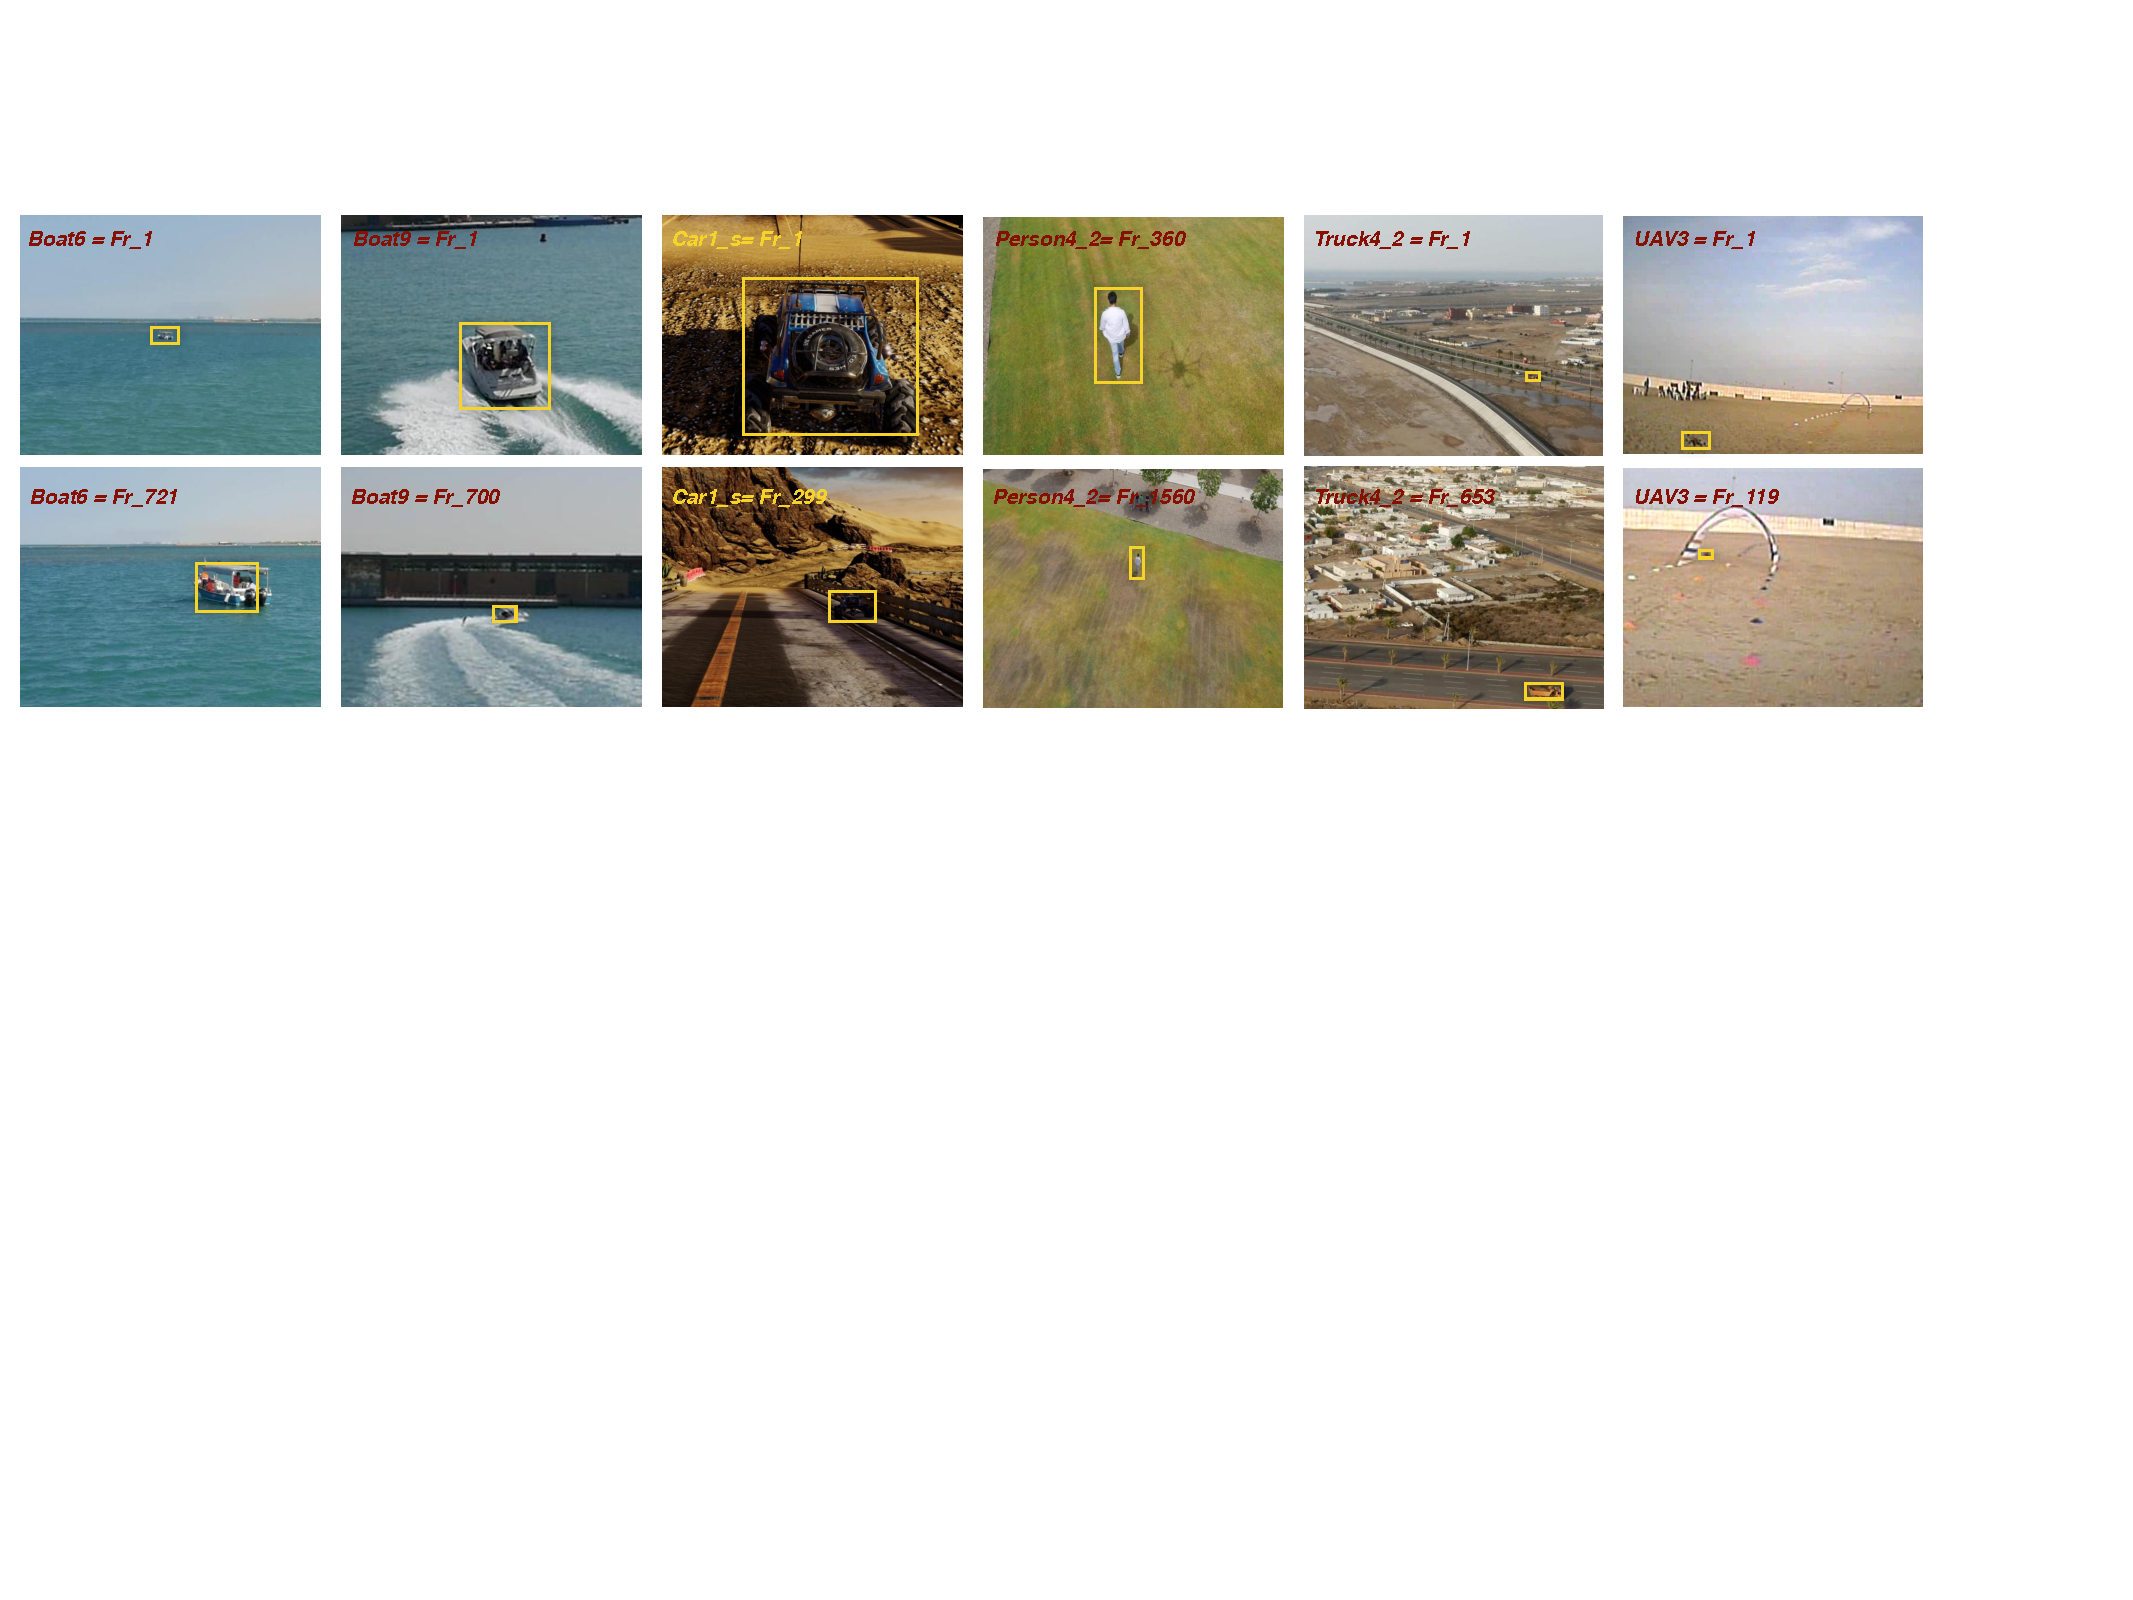
\includegraphics[width=\textwidth]{figures/ResultsIntroduction.pdf}
\caption{Examples of tracking results (yellow rectangles) by the
  proposed method on the ``UAV123'' dataset. This ``UAV123'' dataset
  is challenging for object tracking as a target's scale is changed
  drastically in a few frames.}
\label{ResultsIntroduction}
\end{figure*}

Another way of handling the scale change for the correlation filter
based approach is to estimate a correct scale at a location where a
target highly likely appears \cite{zhang2014fast} -- estimate a
target's translation first and estimate a correct scale afterward. In
particular, Zhang and his colleagues use the MOSSE tracker to estimate
a target's translation. And then they attempted to update the scale of
the target by further analyzing image, sub-regions with high
confidence to figure out the scale of a target. This is based on an
assumption that the scale of a target would not change much over two
consecutive frames. Similarly, Ma and his colleagues used two KCFs to
learn the translation and scale of a target separately
\cite{ma2015long}. In particular, a KCF is used to learn the
translation of the target and its background. Given this, another KCF
is used to learn the target area to estimate a new scale of the
target. However, because of running more than a KCF on each frame,
this method degrades its run-time performance (i.e., $\leq 50
fps$). Our method is motivated by this idea -- the idea of deploying
multiple KCFs to address the issues of single target tracking: scale
and translation, but in a more efficient way. In particular, we use a
multiple of KCFs, in an order of maximizing run-time performance and
accuracy, instead of running them all together on every frame. We
deploy three KCFs in turn: \textit{target}+\textit{small background}
translation filter ($R_{t}^{S}$), \textit{target-only} scale filter
($R_{s}$) and \textit{target}+\textit{large background} translation
filter ($R_{t}^{L}$). By doing so, we could address the scale change
and estimate target's motion efficiently while maintaining or
increasing run-time performance. Figure \ref{fig:Filters} shows
examples of the region of interest (ROI) associated with $R_{t}^{S}$,
$R_{t}^{L}$, and $R_{s}$. Figure \ref{Workflows} illustrates the
work-flow of the {\it E}nKCF.
\begin{figure}[!t]
\centering
\begin{tabular}{cc}
\bmvaHangBox{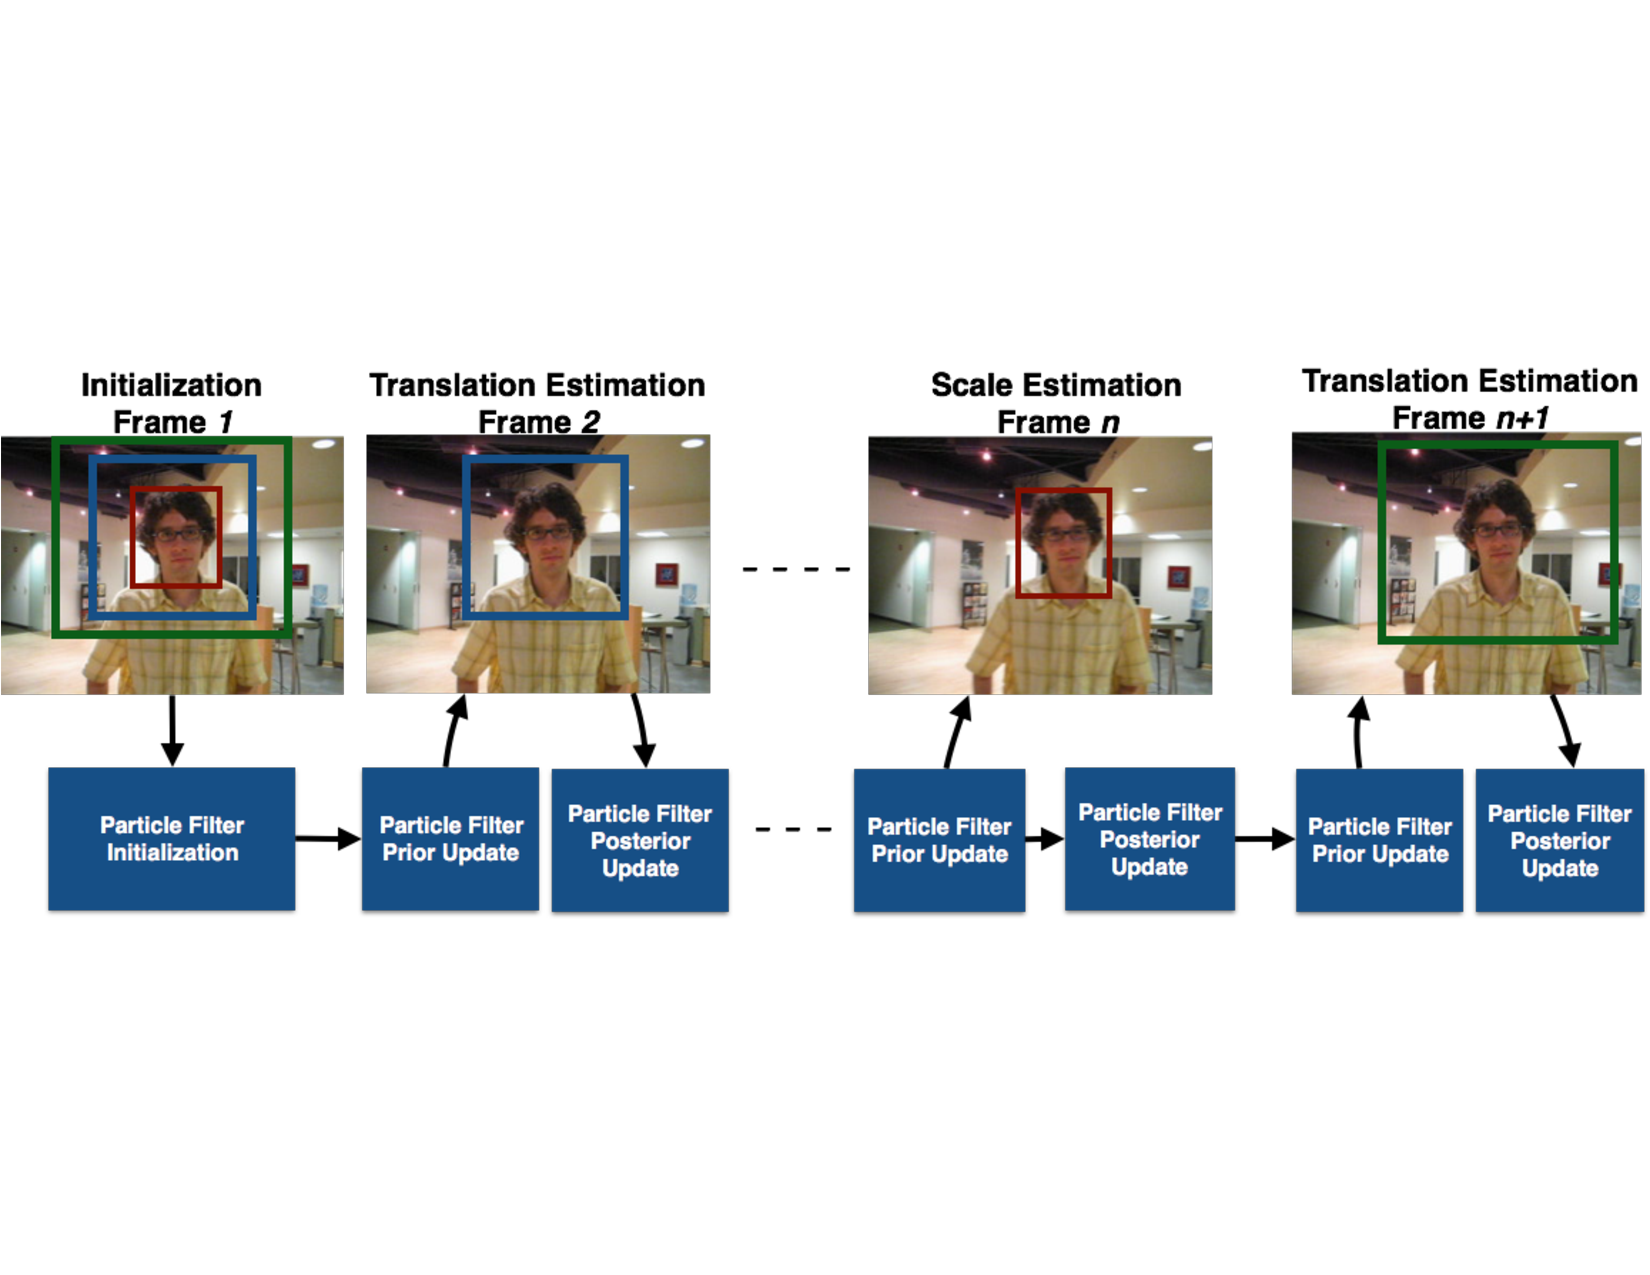
\includegraphics[width=12.00cm]{./figures//Workflow_MKCF+PF.pdf}}\\
\end{tabular}
\caption{The workflow of {\it E}nKCF tracking algorithm. We show the
  first seven frames of tracking where the first frame is the
  initialization frame. Afterward, the order of deploying three KCFs
  is repeating.}
\label{Workflows}
\end{figure}
The contribution of this study is a novel, single-target tracking
algorithm running in a very high-speed, $\geq 300$ fps. In particular,
the proposed algorithm, {\it E}nKCF, deploys an ensemble of KCFs, in
turn, to more effectively address the scale variance and the dynamic
maneuver of a target while preserving run-time performance as high as
possible. To minimize any potential performance gap from transiting
one KCF to another, we use a Bayes filter.

%---------------------------------------------------------------------- 
\section{{\it E}nKCF: Ensemble of Kernelized Correlation Filters}
%---------------------------------------------------------------------- 
In this paper, we propose a novel way of utilizing a multiple of the KCFs
\cite{henriques2015high} to effectively handle scale variations and
dynamic maneuvers of a target. To maintain or improve the run-time
performance of the original KCF (e.g., $\ge$ 300), we deploy three
KCFs in turn, not on the same image frame together. Each of these KCFs
is designed to address specific challenges, i.e., scale and
translation. By alternating their deployments, our algorithm will
improve the performance of the original KCF while preserving the
efficient nature and small-footprint of the KCF computation.

\begin{algorithm}[h]
\small
\DontPrintSemicolon
\KwIn{ Initial bounding box $(x_{0},y_{0},s_{0})$, frame counter $fc$, scale filter frequency $n = 5$,}
\KwOut{	\uIf{$fc\:\%\:n=0$ (\textbf{Condition 1})}
			{
				Estimated Target State $(x_{t},y_{t},s_{t})$,
				Scale filter (\textit{target-only}) model $R_{s}$
			}
			 \ElseIf{$fc\:\%\:n>0\:\:and\:\:fc\:\%\:n\leq n/2$ (\textbf{Condition 2})}
			 {
				Estimated Target State $(x_{t},y_{t},s_{t} = s_{t-1})$,
			  	Large Area Translation Filter model $R_{t}^{L}$
			}			 
			 \Else (\textit{\textbf{Condition 3}})
			{			 
				 Estimated Target State $(x_{t},y_{t},s_{t} = s_{t-1})$,
				Small Area Translation Filter model $R_{t}^{S}$			
			}	
		}
\SetKwBlock{Begin}{function}{end function}
\Begin($\text{track($x_{t-1},y_{t-1},s_{t-1}$) }$)
{
 	// \textit{Translation Estimation - Particle Filter} \\
	Transit Particle Filter to the frame $t$ and compute the mean of prior pdf $\mathbf{(x_{t},y_{t},s_{t-1})}$ \\
     // \textit{Translation Estimation - Correlation Filter} \\
	Crop the ROI for the $R_{t}^{L}$ (Condition 2), or $R_{t}^{S}$ (Condition 3) given $(x_{t},y_{t})$ and estimate new position as $\mathbf{(x_{t},y_{t})}$ = $\mathbf{\textit{max}(y_{R_{t}})}$\\
	// \textit{Scale Estimation - Correlation Filter}\\
	Scale pool for $R_{s}$ : $S = \lbrace1.05,1.0,1/1.05\rbrace$,\\
	Crop the ROI for the $R_{s}^{i}$ (Condition 1) and estimate scale factor, $\mathbf{\alpha}$ = $\mathbf{\underset{i\in S}{\textit{argmax}}(PSR(y_{R_{s}^{i}}))}$, and new scale $\mathbf{s_{t} = \alpha * s_{t-1}}$,\\ 
	Skip it for $R_{t}^{L}$ and $R_{t}^{S}$ ($\mathbf{s_{t}}$=$\mathbf{s_{t-1}}$)\\
	// \textit{Update Translation - Particle Filter}\\
	Do Importance Re-sampling (if necessary) and compute the 
	mean of posterior pdf $\mathbf{(x_{t},y_{t})}$\\
	// \textit{Model Update}\\
	Update $R_{t}^{S}$,\\
	Update $R_{t}^{L}$\\
	\uIf{$PSR(y_{R_{s}}) \geq T_{R_{s}}$}{
		Update $R_{s}$ (Condition 1)}
  \label{endfor}
  \Return{($x_{t},y_{t},s_{t}$)}
}
\caption{{\it E}nKCF Tracking Algorithm}\label{alg:MKCF}
\end{algorithm}

The proposed algorithm, {\it E}nKCF, learns three KCFs in turn: The
first filter, $R_{t}^{S}$, focuses on learning the target area and its
background, \textit{target}+\textit{small background} for addressing a
marginal translation by a target, the second filter, $R_{s}$, focuses
entirely on learning the target's scale, \textit{target-only}, and the
last filter, $R_{t}^{L}$, focuses on the target area and its
background, at least twice, bigger than that of the first filter,
$R_{t}^{S}$, \textit{target}+\textit{large background}. We set up {\it
  E}nKCF in this way because, we believe, a correlation filter for
learning a target's translation should include its background to
better discriminate the target from its surrounding, and another
correlation filter should focus on the target itself to estimate the
right scale of the target. Figure \ref{fig:Filters} shows examples of
the image, sub-regions covered by each of these filters.

\begin{figure}[!h]
\centering
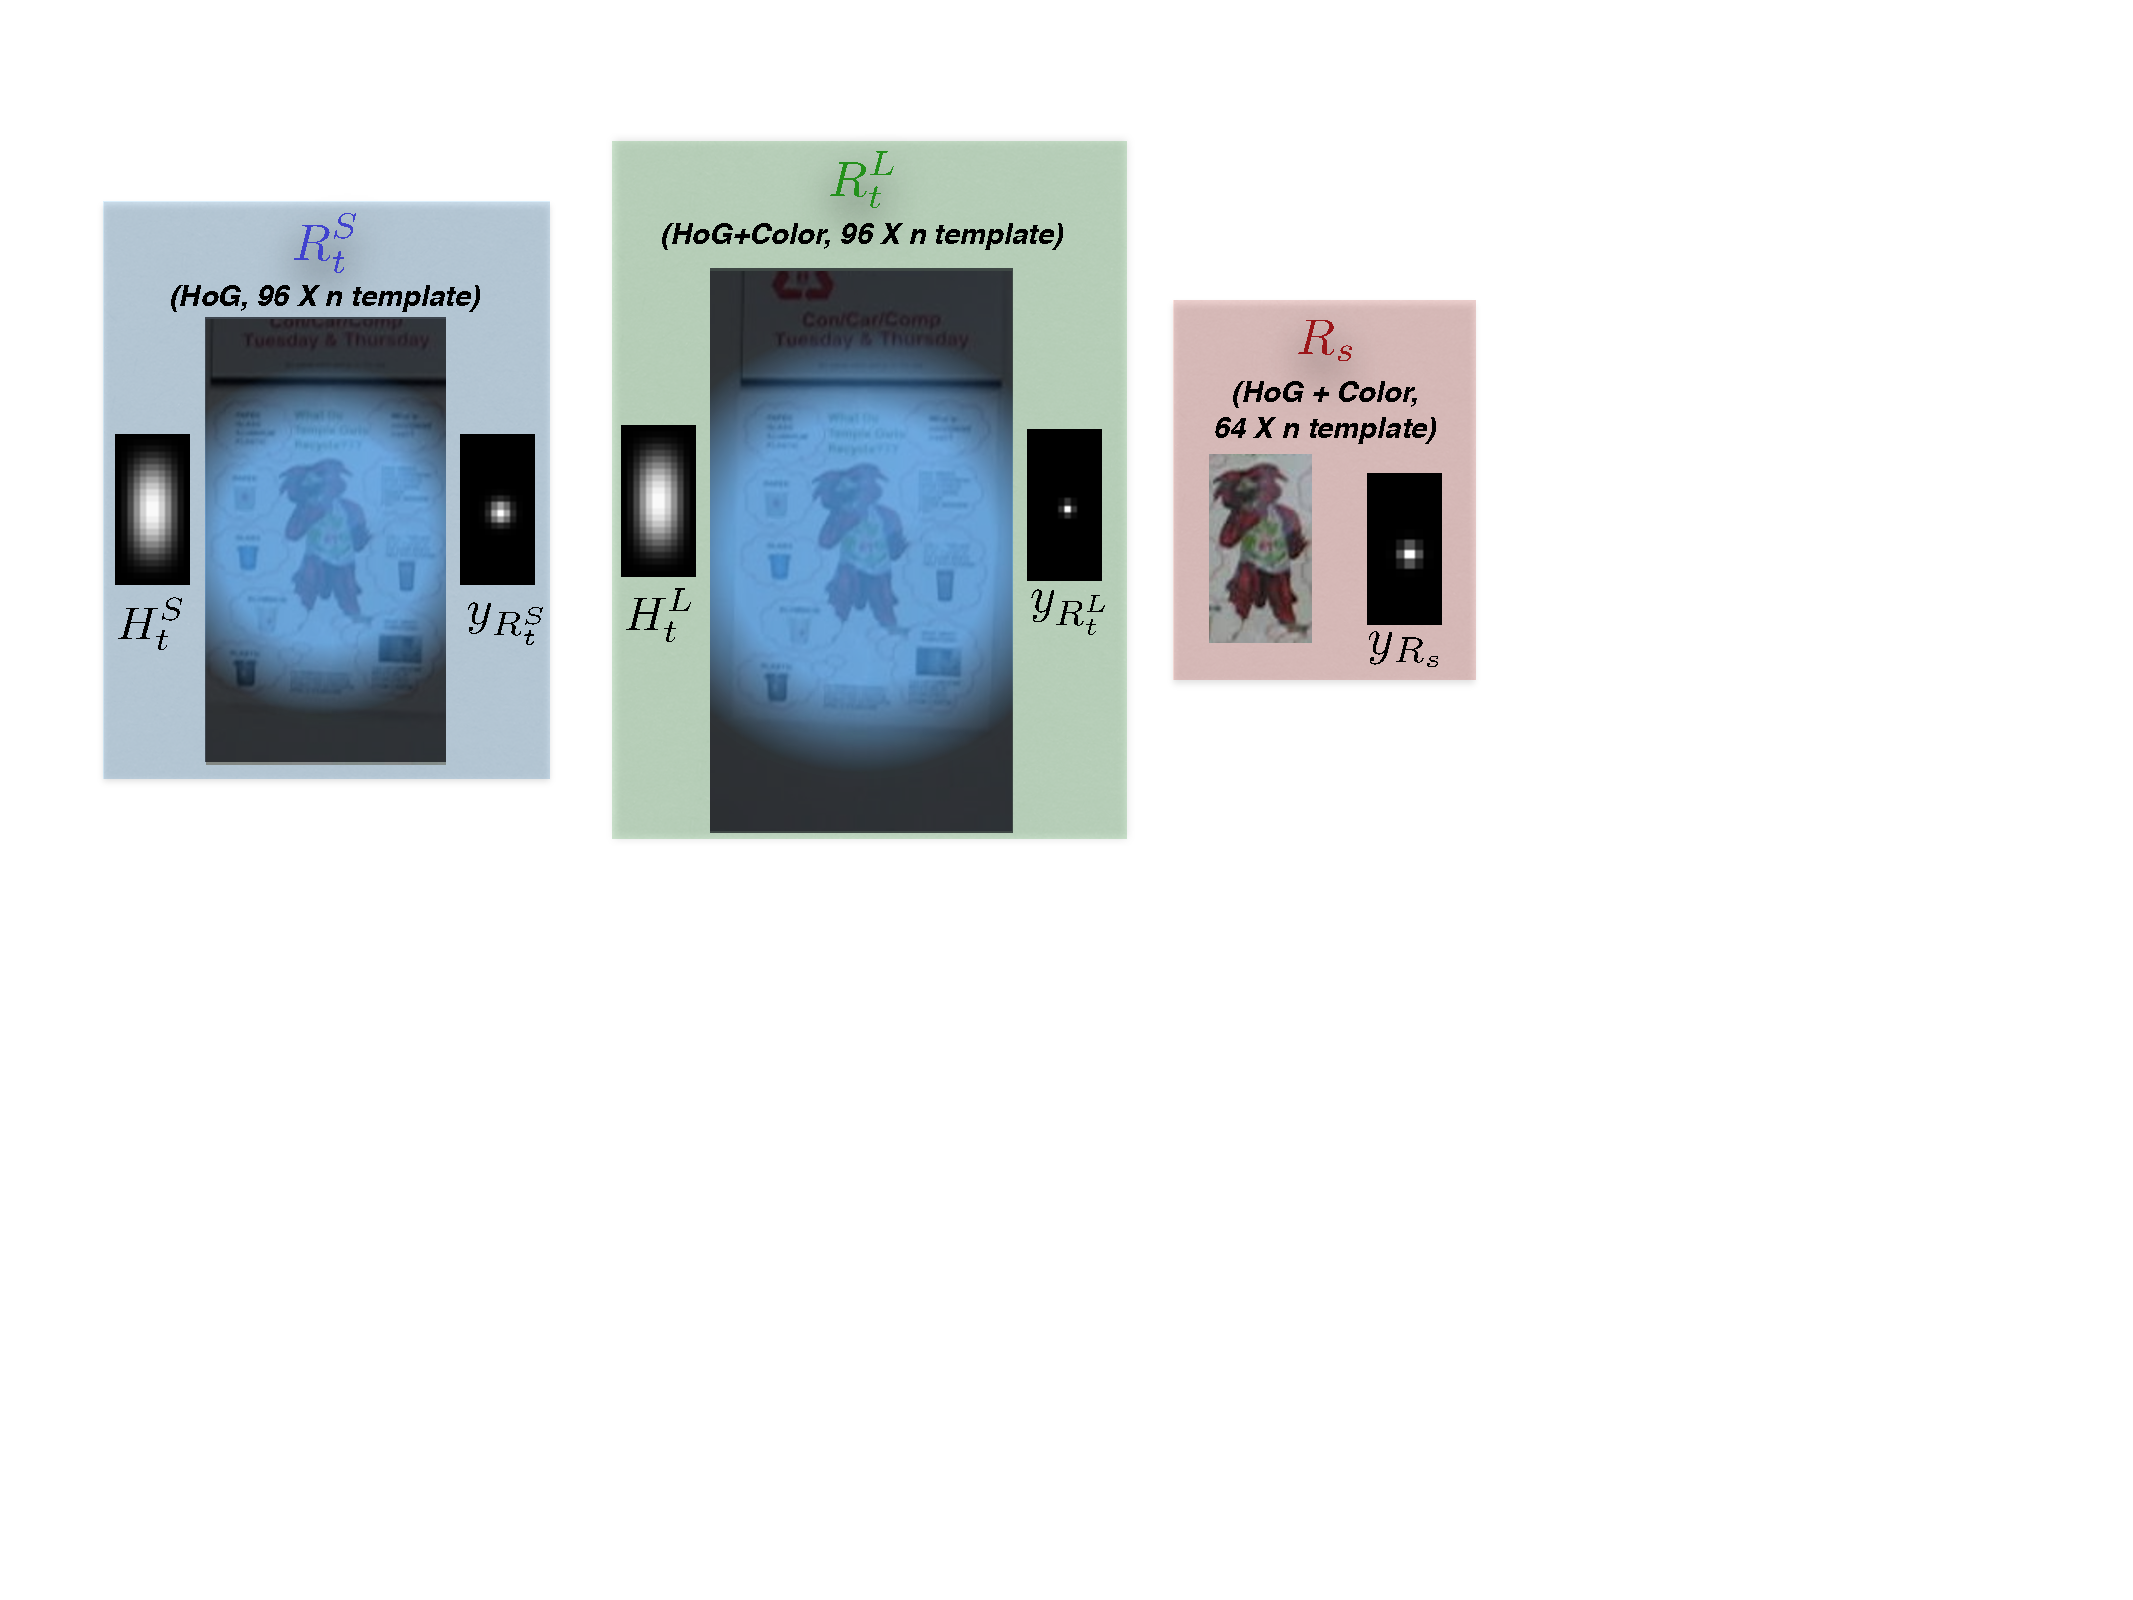
\includegraphics[width=1.0\textwidth]{figures/Filters_Details.pdf}
\caption{Examples of three filters; the translation filter,
  \textit{target+small background}, the scale filter,
  \textit{target-only} and another translation filter,
  \textit{target+large background}, and their Hanning window and
  expected Gaussian response.}
\label{fig:Filters}
\end{figure}

Since Henriques and his colleagues' presented impressive tracking
results of KCF \cite{henriques2015high} on VOT15
challenge \footnote{\url{http://www.votchallenge.net/vot2015/}}, many
variation of KCF were investigated. For example, \cite{ma2015long} and
\cite{danelljan2014accurate} used a scale filter to learn the target
area only whereas \cite{li2014scale, bibi2015multi, tang2015multi}
used a correlation filter learned on the target area and its
surrounding background in different size to learn the optimal scale of
the target. Our approach is similar to that of \cite{ma2015long} in
that more than one KCF is used to address the challenges of single
target tracking. But ours is different from their approach because we
do not use those multiple KCFs together at every frame, but
alternatively at every $k$ frame (e.g., $k=3$). It intuitively makes
sense to alternatively use multiple KCFs with different purposes
because the appearance of a target does not change drastically over
consecutive image frames. For most case, even it looks the appearance
changes, learning a correlation filter over consecutive frames would
not be much different from the one learned using the image few or $k$
frames later. Figure \ref{fig:Filters_Comparison} shows examples
supporting this observation.

\begin{figure}[!h]
\centering
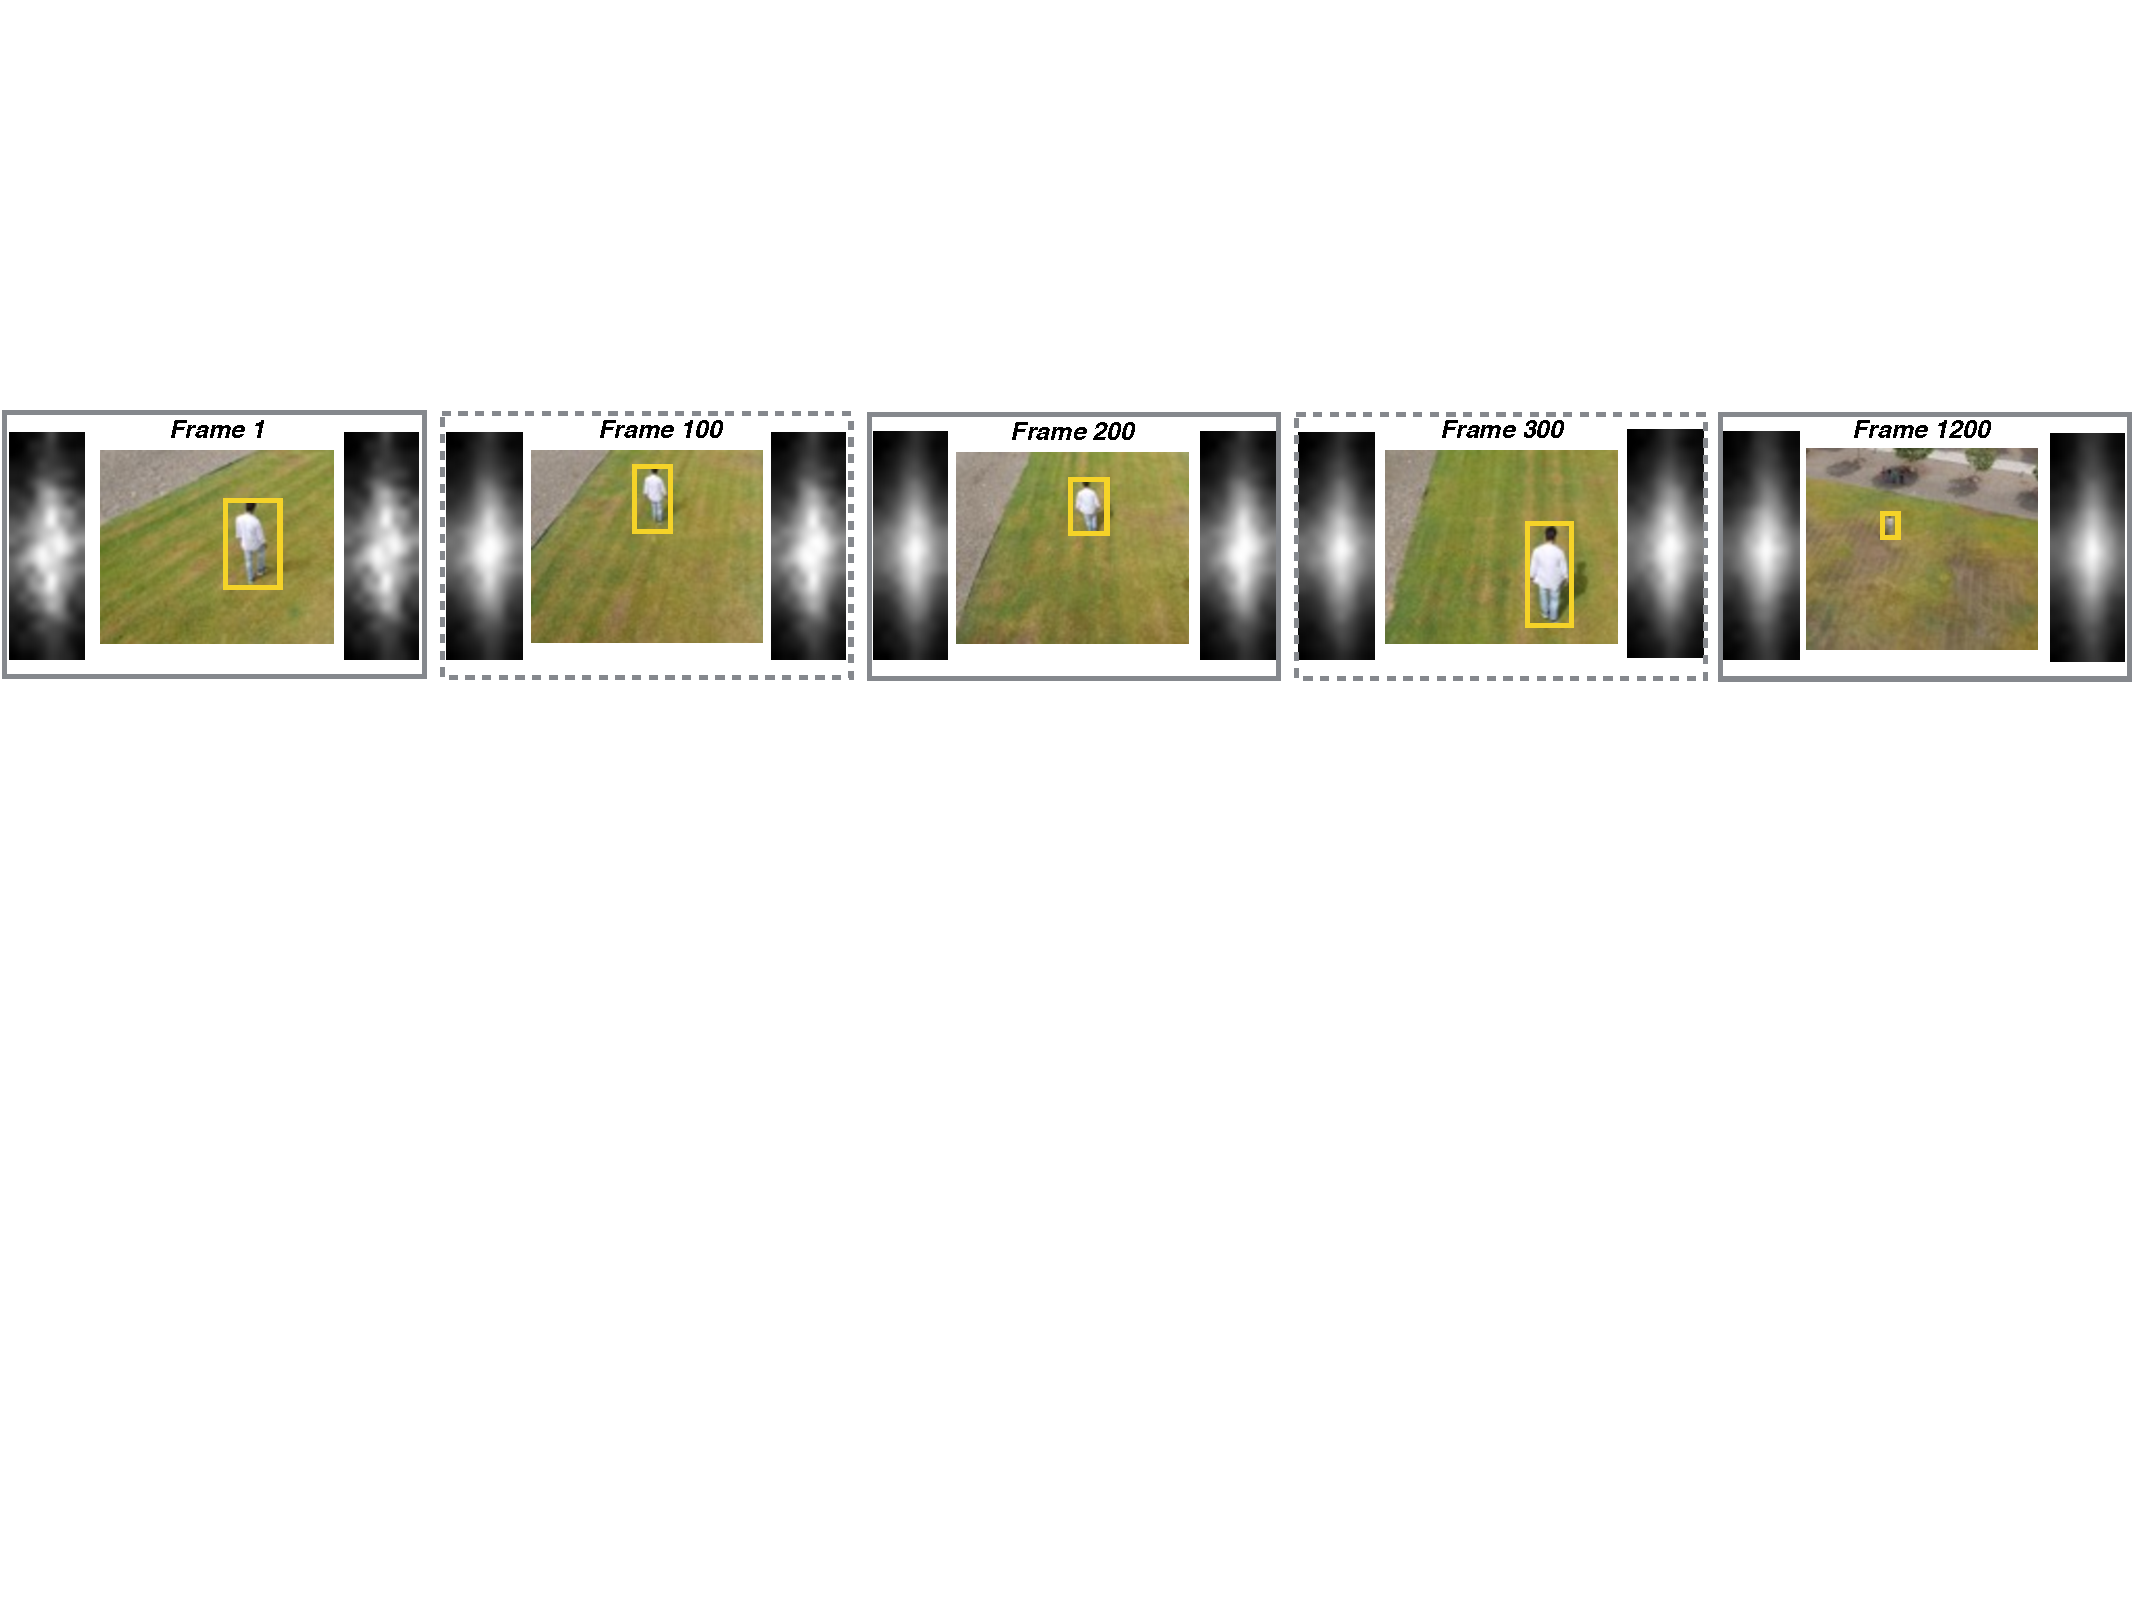
\includegraphics[width=1\textwidth]{figures/LearnedFiltersComparison2.pdf}
\caption{This figure shows that there is marginal difference among the
  scale filters learned either at every frame or at every 5
  frames. The sub-figures at the the left show the scale filters
  trained at every frame and those at the right show the scale
  filters trained at every 5 frames.}
\label{fig:Filters_Comparison}
\end{figure}

The order of running these three KCFs is important because each of
these filters aims at addressing different challenges; The
\textit{target+large background} translation filter, $R_{t}^{L}$, is
applied to the $i$th and $i+1$th image frame, another translation
filter, $R_{t}^{S}$ is applied to the $i+2$th and $i+3$th image frame,
and then the scale filter, $R_{s}$ is applied to the $i+4$the
image. This order repeats until the end of the image frames. The
translation filter, $R_{t}^{L}$, is intended to run right after the
scale filter, $R_s$, runs which is applied at every other $i+4$
frames. We run these filters in this way because we want to minimize
any drifts that are likely to happen running only $R_{s}$. In
addition, the filter, $R_{t}^{S}$, is applied to every other two
frames before $R_{s}$ and right after two consecutive frames running
$R_{t}^{L}$. By repeating this order of learning KCFs, we can
integrate more discriminative shape features that cannot be learned by
$R_{t}^{L}$. This is because it incorporates a large area about
background in the learned model. The filter, $R_{t}^{L}$, uses shape
and color information together to recover from any potential drifts --
drifts could happen only looking the target's scale by the filter,
$R_{s}$.

In summary, the scale filter, $R_{s}$, is designed to directly handle
the scale change of a target and provides $R_{t}^{L}$ and $R_{t}^{S}$
with more focused ROIs about the target's translation. A translation
filter, $R_{t}^{L}$, is intended to look at a larger search area to
estimate the target's translation and recover from any potential
drifts. Another translation filter, $R_{t}^{S}$, on the other hand, is
designed to addresses the drawback of $R_{t}^{L}$ that it may learn
noisy shape features due to its large search area. Figure
\ref{Workflows} illustrates the work-flow of the proposed algorithm
and the algorithm \ref{alg:MKCF} shows the pseudo-code of {\it
  E}nKCF. In the following section, we will briefly describe the
features of the KCF related to this work.

\subsection{Kernelized Correlation Filter} \label{sec:kcf}
The Kernelized Correlation Filter is a well, known single target
tracking method and its work flow has been detailed in other papers
\cite{henriques2012exploiting,henriques2015high}. This section briefly
goes over the parts of the KCF relevant to this study. Its
computational efficiency is derived from the correlation filter
framework representing training examples as a circulant matrix. The
fact that a circulant matrix can be diagonalized by Discrete Fourier
transform is the key to reduce the complexity of any tracking method
based on correlation filter. The off-diagonal elements become zero
whereas the diagonal elements represent the eigenvalues of the
circulant matrix. The egienvalues are equal to the DFT transformation
of the base sample ($x$) elements. The Kernelized Correlation Filter,
in particular, applies a kernel to $x$ to transform to a more
discriminative domain. The circulant matrix is then formed by applying
cyclic shifts on the kernelized $x$. Such kernelization operation maintains 
O($nlog(n)$) complexity unlike other kernel algorithms leading to O($n^{2}$) or even higher 
complexities.

The KCF solves essentially the problem of a regression in the form of
the regularization:
\begin{equation}
E(h) = \frac{1}{2}||y-\sum_{c=1}^{C}h_{c}*x_{c}||^{2} + \frac{\lambda}{2}\sum_{c=1}^{C}||h_{c}||^{2}
\label{eq:Closedform_RidgeReg}
\end{equation}
where $y$ represents the desired continuous response whereas $h$ and
$x_{c}$ represents the learned correlation filter and training
template for the given channel. The parameter $c$ enabled one to
integrate features in multiple channels, such as HoG and color, in
this setup \cite{henriques2015high,galoogahi2013multi}. A closed-form
solution for Equation \ref{eq:Closedform_RidgeReg} exists. To make the
closed-form solution less complex, an element-wise, multiplication in
frequency domain was proposed for $\hat{w}$:
\begin{equation}
\hat{w} = \hat{x}^{*}*\hat{y}(\hat{x}^{*}*\hat{x}+\lambda)^{-1}.
\label{eq:DiagonalizedPrimalSolution}
\end{equation}
A non-linear version of this closed-form solution is proposed to make
it more robust to any geometric and photometric variations
\cite{henriques2015high}. In particular, the diagonalized Fourier
domain dual form solution is expressed as
\begin{equation}
\hat{\alpha} = \hat{y}(\hat{k}^{xx}+\lambda)^{-1}
\label{eq:FourierDualDomainSolution}
\end{equation}
where $\hat{k}^{xx}$ represents the first row of the kernel matrix $K$
known as \textit{gram matrix} and it is expressed as
\begin{equation}
k^{xx^{'}} = exp(-\dfrac{1}{\alpha^{2}}(||x||^{2}+||x^{'}||^{2}-2F^{-1}(\sum^{C}_{c}\hat{x}_{c}^{*}\odot \hat{x}_{c}^{'})))
\label{eq:GaussianCorrelationSingleChannel}
\end{equation}
An early version based on this formulation used grayscale feature
($C=1$) to learn the solution vector $w$ and multi-channel features
such as HoG and Color showed improved accuracy
\cite{henriques2015high,galoogahi2013multi,tang2015multi,ma2015long,bibi2015multi}. Specifically,
one can execute an object detection using this kernelized correlation
filter with multi-channel features as 
\begin{equation}
r(z) = F^{-1}(\hat{k}^{xz} \odot \hat{\alpha})
\end{equation}
where $r$ denotes the correlation response at all cyclic shifts of the
first row of the kernel matrix.

\subsection{Particle Filter for Smoothing Transition among KCFs} \label{sc:PF}
As explained earlier, the {\it E}nKCF updates a target's translation
at every other $k$ frames, particularly for estimating the target's
scale. Although the strategy of updating every other $k$th frames will
result in an optimal run-time performance, this may lead any potential
drifts at the later frames. To prevent such potential drifts, we
developed a Bayes filter that incorporates a target's motion to smooth
any intermediate outputs from individual KCFs of the {\it E}nKCF. In
particular, we use a particle filter to estimate the target's image
coordinate based on the {\it E}nKCF's outputs. A particle filter is a
sequential Monte Carlo method that uses a finite number of particles
or samples to estimate the posterior probability density of a state of
the system \cite{thrun2005probabilistic}. In this study, the state
represents a target's pixel coordinates and its motion. In particular,
the state of the particle filter, $X_t$, is represented by $\lbrace x,
y, v_{x}, v_{y} \rbrace$, where $x$ and $y$ are the pixel coordinates
of the target's centroid, $v_x$ and $v_y$ are the estimated velocity
along the $x$-axis and $y$-axis. The particle filter predicts, using a
constant velocity motion model, a target's state by generating a
predefined number of particles. And then the particle filter uses the
confidence maps of {\it E}nKCF as observation to update the state. The
weight of a particle is computed as, $w_{p_{t}}(x_{t},y_{t}) =
\sum_{i=1}^{N}\sum_{j=1}^{N} y_{R}(x_{t}-i,y_{t}-j)$, where $w_{p}$
denotes the weight of the particle $p$ at time $t$ and $N$ denotes the
size of the window as that of a confidence map. Alternatively one can
also use the Euclidean distance of particles to the location of
maximum response of the confidence map. 
\begin{comment}
We chooses some particles based on their importance to estimate the
target's next state, i.e., its pixel coordinates as $\hat{X}_{t} =
\sum_{p=1}^{P}w_{p_{t}} X_{t}.$ Note that, unlike a typical operation
of a particle filter, we skip the importance re-sampling step when the
scale filter, $R_{s}$, estimates the target's scale change. This is
because we observe the confidence map from the scale filter, $R_s$ is
sometime noisy. In addition, at every iteration, we check the variance
in the velocity components of the particles to re-assign velocities
from uniform initial distribution to keep variance high enough.
\end{comment}

%----------------------------------------------------------------------
\section{Experiments} \label{sc:Experiments}
%---------------------------------------------------------------------- 
To evaluate the performance of the proposed algorithm, we choose two
publicly, available datasets:
OTB100 \footnote{\url{http://cvlab.hanyang.ac.kr/tracker_benchmark/benchmark_v10.html}}
and
UAV123 \footnote{\url{https://ivul.kaust.edu.sa/Pages/Dataset-UAV123.aspx}}\cite{mueller2016uav123}.
The OTB100 dataset is comprised of the videos about 100 objects
whereas UAV123 dataset contains aerial footages of 123 objects. We
aims at developing an object tracking algorithm that ``efficiently''
runs on an embedded system, a drone, for example, in ``high speed,''
$\ge 300$ fps. Given this, we believe that the UAV123 data is a good
fit in evaluating the performance of the proposed algorithm. In
addition, in the UAV123 data, there are many challenging, realistic
scenes, e.g., abrupt scale/illumination changes. Although we are
primarily interested in developing an algorithm for mobile, embedded
robotic applications, it is also important to compare the performance
of the proposed algorithm with those of the state-of-the-art in a
nominal dataset for comparison. To this end, we chose the OTB100 data
that contains the videos recorded from smart phones and typical
cameras in perspective view. Lastly, we tested the proposed algorithm
on a temporally down-sampled version of the UAV123 dataset, called
UAV123$\_$10fps dataset. What we would like to see from this
experiment is to evaluate how robust the proposed algorithm is to
drastic motions of camera and targets.

\textbf{Finding Optimal Hyper-parameters} Each of three KCFs in {\it
  E}nKCF is designed for addressing specific challenges in single,
target tracking problem. Thus each of them should have different
values for the optimal parameters. For instance, the primary task of
the translation filter, $R_{t}^{L}$ is to estimate the translation of
a target from the previous frame whereas the scale filter, $R_{s}$ and
the estimated state of the particle filter are primarily used to
estimate the scale and translation. Because of this, we set the
learning rates ($\beta$) of individual filters, $R_{t}^{L}$,
$R_{t}^{S}$, and $R_{s}$ differently as $0.020$, $0.020$ and
$0.010$. For the kernel of the Gaussian neighboring function, we
empirically found the optimal values of $\alpha$ as $0.6$, $0.4$, and
$0.4$ for $R_{t}^{L}$, $R_{t}^{S}$, and $R_{s}$, and the learning rate
as $0.12$ for $R_{t}^{L}$. For our particle filter implementation, we
empirically set the number of particles to $1000$ to balance the
run-time performance and accuracy. To keep the level of variance among
the particles reasonable, we performed the re-sampling only when the
\textit{efficient number of samples} ($ \hat{N}_{eff} \approx
(\sum_{p=1}^{P}w_{p}^{2})^{-1} $) is lower than a pre-defined
threshold.

\textbf{Features Selections} As each of three KCFs in the {\it E}nKCF
has different goals to accomplish, we used different features for each
of them. In particular, the translation filter, $R_{t}^{L}$, uses both
the fast Histograms of Oriented Gradients (fHoG)
\cite{felzenszwalb2010object} and color-naming \cite{van2009learning}
features to learn the background around the target more
effectively. In fact we empirically found fHoG only didn't work well
to cover the larger ROI. Another translation filter, $R_{t}^{S}$, used
fHoG features only. The scale filter, $R_{s}$ used both fHoG and color
features to learn the scale change more accurately.

\textbf{Performance on UAV123 Dataset} We compared the performance of
the proposed algorithm with those of the state-of-the-art high speed
tracking algorithms by the \textit{Precision} and
\textit{Success\:Rate} metrics. For the precision, we rank the trackers
based on the precision numbers at 20 pixels whereas in the success
rate plots, trackers are ranked based on area under curve (AUC)
scores. The tracking algorithms used for the comparison include ones
in high-speed ($\geq$300 fps), i.e., KCF\cite{henriques2015high}, CSK
\cite{henriques2012exploiting}, DCF\cite{henriques2015high}, and
MOSSE\cite{bolme2010visual,henriques2015high} and ones in relatively
lower-speed ($\geq$50), i.e., SAMF\cite{li2014scale},
DSST\cite{danelljan2014accurate}, Struck\cite{hare2012efficient},
MUSTER \cite{hong2015multi}. TLD \cite{kalal2012tracking}, and OAB
\cite{zhang2012robust}. Figure \ref{fig:UAV123_DATASET} shows the
results on the UAV123 dataset. {\it E}nKCF outperformed most of the
high-speed tracking methods by $3\%$-$15\%$ at 20 pixels precision
metric. Three algorithms, SAMF, DSST, and Struck did about 5\% better
than ours in accuracy, but 10-20\% slower than ours. For the scale
adaptation, {\it E}nKCF did second best in terms of \textit{area under
  curve} (AUC) value for the success rate plot. It outperformed other
tracking methods in high-speed by about $20\%$-$25\%$ in AUC
metric. In addition, it performed even better than those algorithms
that are slow, but a bit better in precision. For example, for AUC,
{\it E}nKCF outperformed Struct and DSST by $5\%$ and $10\%$ while
running at more than $10$ and $30$ times faster.

\textbf{Performance on OTB100 Dataset} Figure \ref{fig:OTB100_DATASET}
shows the results on the OTB100 dataset. Same as with UAV123 dataset,
we observed a similar performance. In particular, {\it E}nKCF showed a
good performance for handling the scale changes. It was the third best
and the second fastest tracking algorithm. For the precision metric,
{\it E}nKCF performed slightly better than most of tracking algorithms
in high-speed trackers. Interestingly, it outperformed another
correlation filter based tracker, DSST, but performing $5\%$ behind of
another low-speed scale adaptive SAMF tracker.
\begin{figure}[!h]
\centering
\begin{tabular}{ccc}
\bmvaHangBox{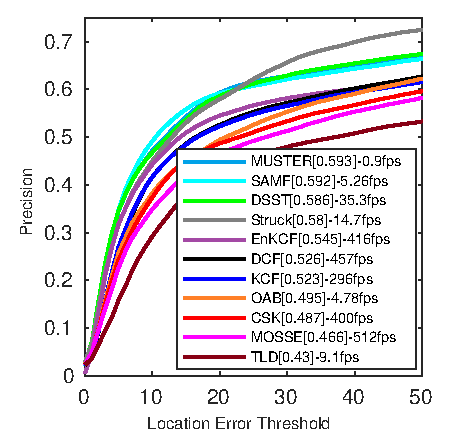
\includegraphics[width=4.80cm]{./figures/Precision_UAV123.eps}}
\bmvaHangBox{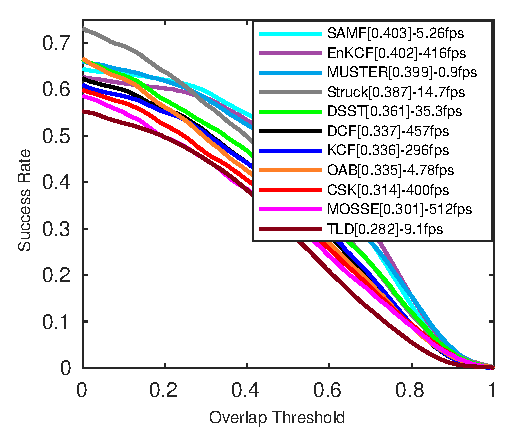
\includegraphics[width=5.30cm]{./figures/Success_UAV123.eps}}
\end{tabular}
\caption{Comparison of {\it E}nKCF's performance with those of the
  state-of-the-art tracking algorithms on the UAV123 dataset.}
\label{fig:UAV123_DATASET}
\end{figure}
\begin{figure}[!h]
\centering
\begin{tabular}{ccc}
\bmvaHangBox{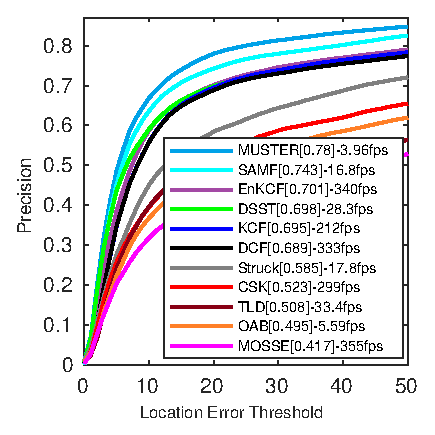
\includegraphics[width=4.80cm]{./figures/Precision_OTB100.eps}}
\bmvaHangBox{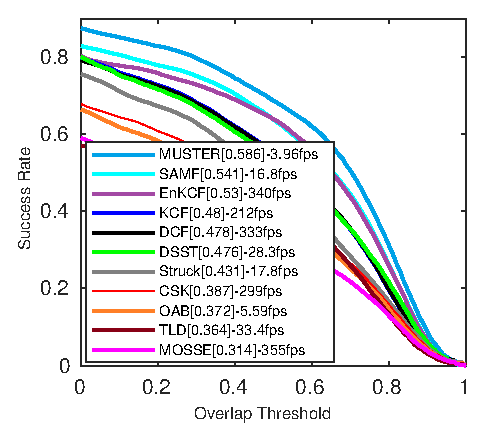
\includegraphics[width=5.30cm]{./figures/Success_OTB100.eps}}\\
\end{tabular}
\caption{Comparison of {\it E}nKCF's performance with those of the
  state-of-the-art tracking algorithms on the OTB100 dataset.}
\label{fig:OTB100_DATASET}
\end{figure}

\textbf{Performance on UAV123$\_$10fps Dataset.} It maybe a slight
digression from the main idea -- the idea of deploying multiple KCFs
to make a very fast and effective, single target tracking
available. We found that, with a slight modification, the proposed
method can effectively handle tracking of object in fast motion and in
large camera motion. Specifically we modified {\it E}nKCF by running
$R_{t}^{L}$ every frame and remove the particle filter instead. We
tested this modified {\it E}nKCF with another vision of the UAV123 that
the original dataset was temporally down-sampled at $10$ fps and makes
the challenging original dataset, because of objects in fast motion
and large ego-motion, more challenging. This is because the magnitude
of those motions is even bigger. Figure \ref{fig:UAV123_10fpsDATASET}
compares the performance of the modified version of {\it E}nKCF and
other tracking methods. Our tracker outperforms other high-speed
correlation filter based trackers including KCF, DSST by about
$15\%$-$20\%$ and showed a precision rate similar to that of SAMF. On
the other hand, it does decent job in scale estimation. It ranks as
second in AUC while running about $150$ faster than the MUSTER
tracker.

\begin{figure}[!h]
\centering
\begin{tabular}{cc}
\bmvaHangBox{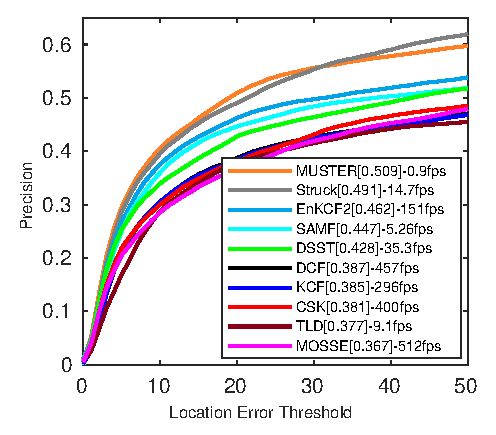
\includegraphics[width=5.30cm]{./figures/Precision_UAV123_10fps.eps}}
\bmvaHangBox{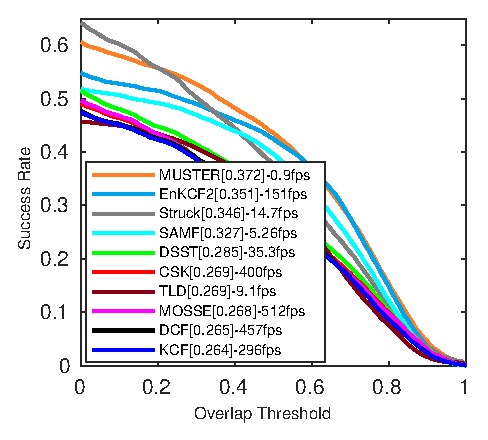
\includegraphics[width=5.30cm]{./figures/Success_UAV123_10fps.eps}}\\
\end{tabular}
\caption{Comparison of a modified {\it E}nKCF's performance with those
  of the state-of-the-art tracking algorithms on the UAV123$\_$10fps
  dataset where the original UAV123 data was temporally downsampled.}
\label{fig:UAV123_10fpsDATASET}
\end{figure}

%---------------------------------------------------------------------- 
\section{Conclusion} \label{sc:Conclusion}
%---------------------------------------------------------------------- 
Running a computer vision algorithm on any existing embedded systems
for real-world applications is economically and practically very
attractive. To make such pipelines more plausible, however, those
algorithms should run faster with small footprint of computation
resource consumption. To make an object tracking algorithm meet these
practical requirements, we proposed an extension of KCF that
essentially deploys three KCFs, in turn, to address the scale change
and dynamic maneuvers of a target. The way we ran three KCFs is
optimal in a sense that efficiently handled the scale change and
effectively learned the translation of the target. We also developed a
Bayes filter, particle filter, to smooth the transition between three
KCFs. In particular, the particle filter estimated the target's pixel
coordinates using information about the target's motion observed over
frames. We used two publicly available dataset to evaluate the
performance of the proposed algorithm and found, on average, the
performance of the proposed algorithm is better than those of the
existing ones over 5\% on precision at 20 pixels and 10-20\% on AUC on
average. Our implementation ran at 340 fps for OTB100 and at 416 fps
for UAV123 data that is faster than DCF (292 fps) for OTB100 and KCF
(292 fps), DCF (457 fps) for UAV123.

As future work, we investigates a way of re-initializing a target when
the target is lost, due to occlusion, illumination change, drastic
camera motion, etc.
%--------------
%\section*{Acknowledgements}
%put stuff here for the accepted , but not the ICCV version

\bibliography{draft}
\end{document}
